% =============================================================================
% relatorio_contador.tex -- Contador Sincrono de 4 bits
% Unidade 5 | Capitulo 3 | Capacitacao Profissional em Microeletronica (PADIS)
% Autor : Matheus Serrao Uchoa   Matricula: 22052633
% Prof. : Thiago Brito
% =============================================================================
\documentclass[12pt,a4paper]{article}

\usepackage[utf8]{inputenc}
\usepackage[T1]{fontenc}
\usepackage[brazil]{babel}
\usepackage{lmodern}
\usepackage{geometry}
\usepackage{graphicx}
\usepackage{booktabs}
\usepackage{array}
\usepackage{multirow}
\usepackage{amsmath}
\usepackage{xcolor}
\usepackage{hyperref}
\usepackage{fancyhdr}
\usepackage{titlesec}
\usepackage{caption}
\usepackage{float}
\usepackage{enumitem}
\usepackage[most]{tcolorbox}
\usepackage{listings}
\usepackage{tikz}
\usetikzlibrary{arrows.meta, positioning, shapes.geometric, fit, calc}

\geometry{top=2.5cm, bottom=2.5cm, left=3cm, right=2.5cm}

% ---------------------------------------------------------------------------
% Cores
% ---------------------------------------------------------------------------
\definecolor{azulpadis}{RGB}{0,82,155}
\definecolor{verdepadis}{RGB}{0,130,79}
\definecolor{cinzaclaro}{RGB}{245,245,245}
\definecolor{cinzaborda}{RGB}{180,180,180}
\definecolor{codebg}{RGB}{252,252,252}
\definecolor{codeframe}{RGB}{180,180,200}
\definecolor{kw}{RGB}{0,0,180}
\definecolor{cm}{RGB}{60,120,60}
\definecolor{st}{RGB}{163,21,21}

% ---------------------------------------------------------------------------
% Cabecalho e rodape
% ---------------------------------------------------------------------------
\pagestyle{fancy}
\fancyhf{}
\fancyhead[L]{\small\textcolor{azulpadis}{\textbf{PADIS -- Microeletronica}}}
\fancyhead[R]{\small\textcolor{azulpadis}{Unidade 5 | Cap.\ 3 -- Contador Sincrono}}
\fancyfoot[C]{\small\thepage}
\renewcommand{\headrulewidth}{0.4pt}

% ---------------------------------------------------------------------------
% Titulos
% ---------------------------------------------------------------------------
\titleformat{\section}{\large\bfseries\color{azulpadis}}{{\thesection.}}{0.5em}{}[\titlerule]
\titleformat{\subsection}{\normalsize\bfseries\color{azulpadis}}{{\thesubsection}}{0.5em}{}
\titleformat{\subsubsection}{\normalsize\bfseries\color{verdepadis}}{{\thesubsubsection}}{0.5em}{}

% ---------------------------------------------------------------------------
% tcolorbox
% ---------------------------------------------------------------------------
\tcbuselibrary{skins, breakable}

\newtcolorbox{destaquebox}[1][]{
  enhanced, breakable,
  colback=cinzaclaro, colframe=azulpadis,
  fonttitle=\bfseries\small, title=#1,
  boxrule=0.6pt, arc=3pt,
  left=4pt, right=4pt, top=4pt, bottom=4pt
}

\newtcolorbox{unidadebox}[1][]{
  enhanced, breakable,
  colback=blue!4!white, colframe=azulpadis!70,
  fonttitle=\bfseries\small\color{azulpadis},
  title=#1,
  boxrule=0.5pt, arc=3pt,
  left=5pt, right=5pt, top=4pt, bottom=4pt
}

% ---------------------------------------------------------------------------
% Listings -- SystemVerilog
% ---------------------------------------------------------------------------
\lstdefinelanguage{SystemVerilog}{
  morekeywords={module,endmodule,parameter,input,output,logic,always_comb,
    always_ff,typedef,enum,posedge,negedge,begin,end,case,endcase,
    unique,if,else,default,assign,wire,reg,int,initial,task,endtask,
    automatic,timescale,forever,repeat,monitor,display,finish,dumpfile,
    dumpvars,error,assert},
  sensitive=true,
  morecomment=[l]{//},
  morecomment=[s]{/*}{*/},
  morestring=[b]"
}

\lstset{
  language=SystemVerilog,
  backgroundcolor=\color{codebg},
  frame=single,
  rulecolor=\color{codeframe},
  basicstyle=\ttfamily\footnotesize,
  keywordstyle=\color{kw}\bfseries,
  commentstyle=\color{cm}\itshape,
  stringstyle=\color{st},
  numbers=left,
  numberstyle=\tiny\color{gray},
  numbersep=6pt,
  tabsize=4,
  breaklines=true,
  showstringspaces=false,
  captionpos=b,
  xleftmargin=12pt,
  xrightmargin=4pt
}

% ===========================================================================
\begin{document}

% ---------------------------------------------------------------------------
% CAPA
% ---------------------------------------------------------------------------
\begin{titlepage}
  \centering
  \vspace*{1cm}

  {\Large\bfseries\color{azulpadis}
    Programa de Apoio ao Desenvolvimento da Indústria de Semicondutores\\[4pt]
    \textsc{PADIS} -- Capacitação em Microeletrônica}

  \vspace{0.4cm}
  \textcolor{cinzaborda}{\rule{\linewidth}{1.2pt}}
  \vspace{0.8cm}

  {\LARGE\bfseries Unidade 5 | Capítulo 3\\[6pt]
   Contador Síncrono de 4 Bits\\[4pt]
   Reset Assíncrono e Enable Síncrono}

  \vspace{0.8cm}
  \textcolor{cinzaborda}{\rule{\linewidth}{0.6pt}}

  \vspace{1.0cm}
  \begin{center}
    \begin{tikzpicture}[node distance=1.4cm, >=Stealth,
        blk/.style={draw=azulpadis, thick, rounded corners=4pt,
                    minimum width=2.2cm, minimum height=0.9cm,
                    font=\small, fill=blue!6, align=center}]

      \node[blk] (ff) {Flip-Flop\\D (x4)};
      \node[blk, right=2cm of ff] (inc) {Somador\\count+1};
      \node[blk, above=of ff, minimum width=1.4cm, fill=verdepadis!15,
            draw=verdepadis] (rst) {rst\_n};
      \node[blk, below=of ff, minimum width=1.4cm] (en) {en};

      \draw[->] (ff)  -- node[above, font=\tiny]{count} (inc);
      \draw[->] (inc) -- ++(2,0) node[right, font=\small]{count+1}
                      -- ++(0,-2.5) -| (ff);
      \draw[->] (rst) -- node[left, font=\tiny]{async} (ff);
      \draw[->] (en)  -- node[right, font=\tiny]{sync}  (ff);

      \node[left=1.2cm of ff, font=\small] (clk) {clk};
      \draw[->] (clk) -- (ff);
    \end{tikzpicture}
  \end{center}

  \vspace{0.8cm}
  \textcolor{cinzaborda}{\rule{\linewidth}{0.6pt}}
  \vspace{0.8cm}

  \begin{tabular}{rl}
    \textbf{Aluno:} & Matheus Serrão Uchôa -- Matrícula: 22052633 \\[4pt]
    \textbf{Professor:} & Thiago Brito \\[4pt]
    \textbf{Curso:} & Capacitação Profissional em Microeletrônica (PADIS) \\[4pt]
    \textbf{Instituição:} & Universidade Federal do Amazonas (UFAM) \\[4pt]
    \textbf{Data:} & Maio de 2026
  \end{tabular}
\end{titlepage}

\tableofcontents
\newpage

% ===========================================================================
\section{Introdução}
% ===========================================================================

Contadores síncronos são componentes fundamentais em sistemas digitais, presentes
em divisores de frequência, temporizadores, sequenciadores de controle, endereçadores
de memória e interfaces de comunicação. O domínio de sua implementação em linguagens
de descrição de hardware é uma competência essencial no projeto de circuitos integrados.

Este relatório documenta o projeto e verificação de um \textbf{contador síncrono de
4 bits} em SystemVerilog IEEE 1800-2012, com as seguintes funcionalidades:

\begin{itemize}[leftmargin=1.5cm]
  \item \textbf{Contagem crescente} (\textit{up-counter}): incrementa em 1 a cada
        borda de subida do clock;
  \item \textbf{Reset assíncrono ativo em nível baixo} (\texttt{rst\_n}): zera o
        contador imediatamente, independente do clock;
  \item \textbf{Enable síncrono ativo em nível alto} (\texttt{en}): o incremento
        só ocorre na borda do clock se \texttt{en = 1};
  \item \textbf{Overflow natural}: ao atingir 15 (\texttt{4'b1111}), o próximo
        incremento retorna automaticamente a 0.
\end{itemize}

\begin{unidadebox}[Conexao com o Curso -- Unidade 5 / Capitulo 3: Consideracoes de Clock]
  O contador síncrono exemplifica os conceitos de clock, reset assíncrono e enable
  síncrono abordados no Capítulo 3. O uso de atribuições \textit{nonblocking} (\texttt{<=})
  dentro do bloco \texttt{always\_ff} segue a prática recomendada para descrever
  lógica sequencial, simulando o comportamento real de flip-flops D.
\end{unidadebox}

% ===========================================================================
\section{Objetivos}
% ===========================================================================

\begin{itemize}[leftmargin=1.5cm]
  \item Implementar o módulo \texttt{sync\_counter} com interface
        \texttt{clk}, \texttt{rst\_n}, \texttt{en} e \texttt{count[3:0]};
  \item Utilizar \texttt{always\_ff} com atribuições \textit{nonblocking} (\texttt{<=});
  \item Verificar todas as funcionalidades por meio de testbench completo com
        \texttt{\$monitor}, verificações \texttt{PASS/FAIL} e dump VCD;
  \item Cobrir os cenários: reset assíncrono, contagem 0→15→0 (overflow),
        enable/disable, toggle do enable e reset durante contagem ativa.
\end{itemize}

% ===========================================================================
\section{Materiais e Ferramentas}
% ===========================================================================

\begin{table}[H]
  \centering
  \caption{Ferramentas utilizadas}
  \label{tab:ferramentas}
  \begin{tabular}{lll}
    \toprule
    \textbf{Ferramenta} & \textbf{Versão} & \textbf{Finalidade} \\
    \midrule
    Icarus Verilog (iverilog) & 12.0 & Compilação SystemVerilog (\texttt{-g2012}) \\
    VVP runtime               & 12.0 & Simulação / geração de VCD \\
    GTKWave / EPWave          & 3.3  & Visualização das formas de onda \\
    Python / Matplotlib       & 3.11 / 3.8 & Geração de figuras para o relatório \\
    \LaTeX\ (pdflatex)        & TeX Live 2023 & Composição deste relatório \\
    \bottomrule
  \end{tabular}
\end{table}

% ===========================================================================
\section{Fundamentos Teóricos}
% ===========================================================================

\subsection{Contador Síncrono}

Em um contador \textbf{síncrono}, todos os flip-flops são acionados pela mesma
borda de clock. Isso elimina os \textit{ripple delays} presentes em contadores
assíncronos, tornando a operação mais rápida e previsível para síntese.

A arquitetura do contador de 4 bits é composta por:
\begin{itemize}[leftmargin=1.5cm]
  \item Quatro flip-flops D formando o registrador de 4 bits (\texttt{count[3:0]});
  \item Um somador combinacional que calcula \texttt{count + 1};
  \item Lógica de controle para \texttt{rst\_n} (assíncrono) e \texttt{en} (síncrono).
\end{itemize}

\subsection{Reset Assíncrono vs.\ Enable Síncrono}

\begin{table}[H]
  \centering
  \caption{Diferença entre reset assíncrono e enable síncrono}
  \label{tab:async_vs_sync}
  \begin{tabular}{lll}
    \toprule
    \textbf{Sinal} & \textbf{Tipo} & \textbf{Comportamento} \\
    \midrule
    \texttt{rst\_n} & Assíncrono, ativo baixo &
      Zera \texttt{count} imediatamente, sem esperar borda \\
    \texttt{en}     & Síncrono, ativo alto    &
      Habilita incremento apenas na borda de subida do clock \\
    \bottomrule
  \end{tabular}
\end{table}

A sensibilidade do bloco \texttt{always\_ff} à \texttt{negedge rst\_n} garante
que o reset seja tratado de forma assíncrona pelo sintetizador, mapeando
corretamente para o pino \textit{clear} assíncrono dos flip-flops.

\subsection{Atribuições Nonblocking (\texttt{<=})}

Atribuições \textit{nonblocking} em blocos \texttt{always\_ff} simulam
o comportamento dos flip-flops: todos os lados direitos são avaliados
primeiro, depois os lados esquerdos são atualizados simultaneamente.
Isso evita condições de corrida em lógica sequencial, conforme especificado
no material do Capítulo 3, Seção 4.2:

\begin{quote}
  \itshape ``Atribuições Nonblocking (\texttt{<=}): Simulam a lógica sequencial,
  como flip-flops.''
\end{quote}

\subsection{Overflow Natural de 4 Bits}

Com 4 bits de largura, \texttt{count} assume valores de 0 a 15. A instrução
\texttt{count <= count + 1'b1} em SystemVerilog produz overflow natural:
ao incrementar 15 (\texttt{4'b1111}), o somador gera 16 (\texttt{5'b10000}),
mas os 4 bits inferiores resultam em \texttt{4'b0000} -- portanto o contador
retorna automaticamente a 0 sem lógica adicional.

% ===========================================================================
\section{Implementação em SystemVerilog}
% ===========================================================================

\subsection{Módulo \texttt{sync\_counter.sv}}

\lstinputlisting[
  caption={sync\_counter.sv -- Contador Síncrono de 4 bits},
  label={lst:counter}
]{sync_counter.sv}

O módulo apresenta apenas \textbf{8 linhas de lógica efetiva}, demonstrando a
expressividade do SystemVerilog para descrição de hardware sequencial. O
\texttt{always\_ff} é sensível a:
\begin{itemize}[leftmargin=1.5cm]
  \item \texttt{posedge clk} -- borda de subida para operação síncrona;
  \item \texttt{negedge rst\_n} -- borda de descida para reset assíncrono imediato.
\end{itemize}

\subsection{Diagrama de Blocos}

\begin{figure}[H]
  \centering
  \begin{tikzpicture}[node distance=1.8cm, >=Stealth,
      blk/.style={draw=azulpadis, thick, rounded corners=5pt,
                  minimum width=2.8cm, minimum height=1.0cm,
                  font=\small\ttfamily, fill=blue!6, align=center},
      mux/.style={draw=azulpadis, thick, trapezium,
                  trapezium left angle=70, trapezium right angle=110,
                  minimum height=1.0cm, font=\small, fill=cinzaclaro}]

    \node[blk] (reg) {Registrador\\count[3:0]};
    \node[blk, right=3cm of reg] (add) {Somador\\+1};
    \node[mux, right=2.2cm of add] (mux) {MUX\\en};

    \draw[->] (reg) -- node[above, font=\tiny]{count} (add);
    \draw[->] (add) -- node[above, font=\tiny]{count+1} (mux);
    \draw[->] (mux) -- ++(1.5,0) node[right,font=\footnotesize]{count\_next}
                    -- ++(0,-2) -| node[above left, font=\tiny]{D} (reg);

    % rst_n
    \node[above=1.2cm of reg, font=\small\ttfamily] (rst) {rst\_n (async)};
    \draw[->, dashed, color=verdepadis] (rst) -- (reg);

    % clk
    \node[left=1.5cm of reg, font=\small\ttfamily] (clk) {clk};
    \draw[->] (clk) -- (reg);

    % en
    \node[above=0.6cm of mux, font=\small\ttfamily] (en) {en};
    \draw[->] (en) -- (mux);

    % count output
    \node[below=0.5cm of reg, font=\small\ttfamily] {count[3:0]};
    \draw[->] (reg) -- ++(0,-0.8);
  \end{tikzpicture}
  \caption{Diagrama de blocos do contador síncrono de 4 bits}
  \label{fig:blocos}
\end{figure}

% ===========================================================================
\section{Testbench}
% ===========================================================================

\subsection{Cobertura de Verificação}

O testbench \texttt{tb\_sync\_counter.sv} cobre os seguintes cenários,
organizados em 7 testes sequenciais:

\begin{table}[H]
  \centering
  \caption{Cenários de verificação do testbench}
  \label{tab:testes}
  \begin{tabular}{clp{7cm}}
    \toprule
    \textbf{Teste} & \textbf{Cenário} & \textbf{Verificação} \\
    \midrule
    1 & Reset assíncrono inicial       & \texttt{count = 0} imediatamente (sem borda de clock) \\
    2 & Contagem com \texttt{en=1}     & Sequência 0→1→2→3→4→5→6→7 verificada \\
    3 & Enable desativado (\texttt{en=0}) & \texttt{count} congela em 7 por 3 ciclos \\
    4 & Reativação do enable            & Retoma de 7→8→9→10 \\
    5 & Toggle do enable                & Alterna entre contar e congelar \\
    6 & Overflow (\texttt{15→0})        & count=15, próximo ciclo count=0 \\
    7 & Reset assíncrono mid-cycle      & Reset no meio de ciclo zera imediatamente \\
    \bottomrule
  \end{tabular}
\end{table}

\subsection{Código do Testbench}

\lstinputlisting[
  caption={tb\_sync\_counter.sv -- Testbench completo},
  label={lst:tb}
]{tb_sync_counter.sv}

% ===========================================================================
\section{Resultados de Simulação}
% ===========================================================================

\subsection{Compilação}

\begin{lstlisting}[language=bash, caption={Compilação e execução},
                   label={lst:cmd}, numbers=none]
iverilog -g2012 -o sim_counter sync_counter.sv tb_sync_counter.sv
vvp sim_counter
\end{lstlisting}

\subsection{Saída do Console}

\begin{lstlisting}[language={},
  caption={Log completo da simulação (26/26 verificações corretas)},
  label={lst:log},
  numbers=none, frame=single, backgroundcolor=\color{cinzaclaro},
  basicstyle=\ttfamily\scriptsize]
========================================================
  Simulacao: Contador Sincrono 4 bits
  Sequencia: rst_n / enable / disable / overflow / reset
========================================================

--- TESTE 1: Reset assincrono (rst_n = 0) ---
  [OK]    Reset assincrono imediato: count=0

--- TESTE 2: Enable sincrono (en=1), conta 0->7 ---
  [OK]    en=1, ciclo  1 | count=1
  [OK]    en=1, ciclo  2 | count=2
  [OK]    en=1, ciclo  3 | count=3
  [OK]    en=1, ciclo  4 | count=4
  [OK]    en=1, ciclo  5 | count=5
  [OK]    en=1, ciclo  6 | count=6
  [OK]    en=1, ciclo  7 | count=7

--- TESTE 3: Enable desativado (en=0), count congela em 7 ---
  [OK]    en=0, ciclo  1 (congela) | count=7
  [OK]    en=0, ciclo  2 (congela) | count=7
  [OK]    en=0, ciclo  3 (congela) | count=7

--- TESTE 4: Reativa en=1, continua de 7 ---
  [OK]    en=1 reativado, count=8 | count=8
  [OK]    en=1, count=9  | count=9
  [OK]    en=1, count=10 | count=10

--- TESTE 5: Toggle en durante contagem ---
  [OK]    en=0, count congela 10 | count=10
  [OK]    en=1, count=11         | count=11
  [OK]    en=0, count congela 11 | count=11
  [OK]    en=1, count=12         | count=12

--- TESTE 6: Overflow (15 -> 0) ---
  [OK]    count=13        | count=13
  [OK]    count=14        | count=14
  [OK]    count=15 (maximo)| count=15
  [OK]    overflow: count=0| count=0
  [OK]    pos-overflow: count=1 | count=1

--- TESTE 7: Reset assincrono durante contagem ativa ---
  [OK]    Reset assincrono mid-cycle: count=0 imediato
  [OK]    apos reset, continua contagem: count=1 | count=1
  [OK]    count=2 | count=2

========================================================
  Acertos: 26 | Erros: 0
  >>> RESULTADO: APROVADO <<<
  Simulacao concluida em 286000
========================================================
\end{lstlisting}

\subsection{Formas de Onda}

\begin{figure}[H]
  \centering
  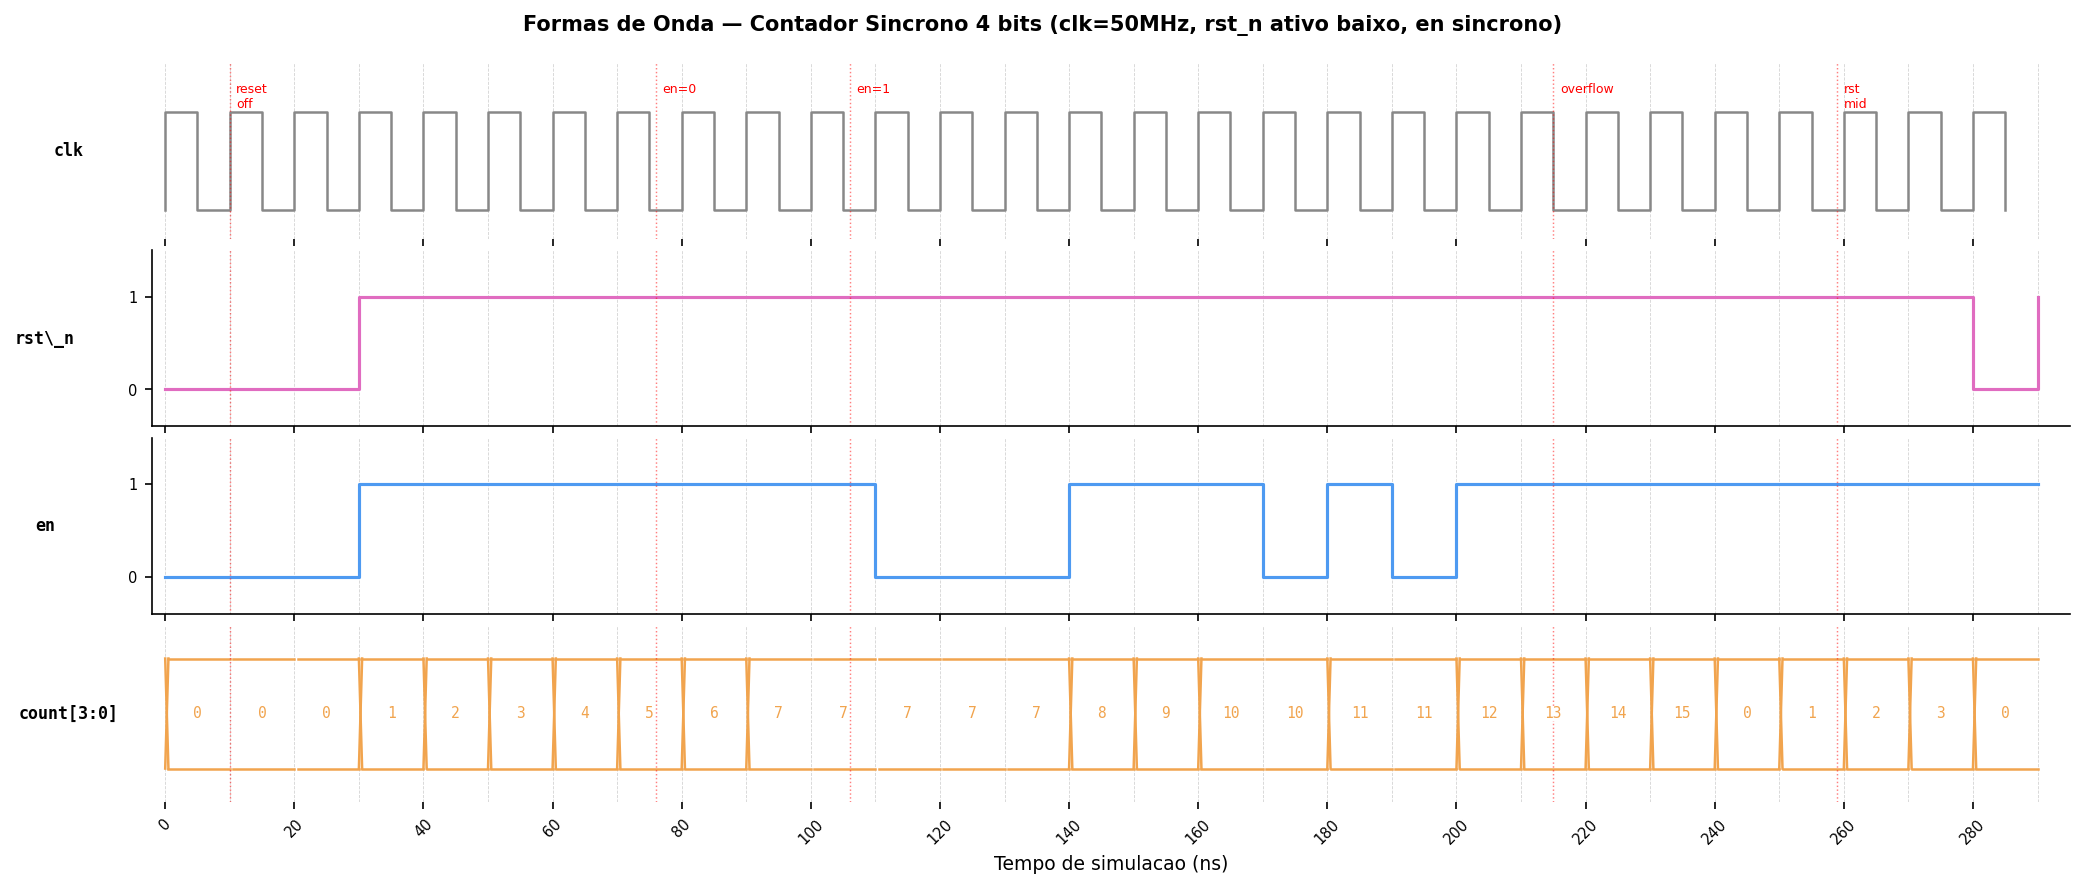
\includegraphics[width=\textwidth]{fig_waveform_counter.png}
  \caption{Formas de onda do Contador Síncrono 4 bits. As linhas pontilhadas
           vermelhas marcam os eventos-chave: desativação do reset, toggle do
           enable, overflow (count: 15→0) e reset assíncrono mid-cycle.}
  \label{fig:wave}
\end{figure}

\subsection{Análise dos Resultados}

\subsubsection{Reset Assíncrono}

O teste 1 e o teste 7 confirmam que \texttt{rst\_n = 0} zera \texttt{count}
\emph{imediatamente}, sem aguardar a próxima borda de clock. Isso é garantido
pela sensibilidade do \texttt{always\_ff} à \texttt{negedge rst\_n}.

\subsubsection{Enable Síncrono}

Os testes 2, 3 e 5 verificam que o contador somente incrementa na borda do
clock \emph{quando} \texttt{en = 1}. Com \texttt{en = 0}, o valor de
\texttt{count} permanece inalterado por quantos ciclos forem necessários.

\subsubsection{Overflow Natural}

O teste 6 demonstra que ao atingir 15 (\texttt{4'b1111}), a operação
\texttt{count + 1'b1} resulta em \texttt{4'b0000} por truncamento natural
de 4 bits -- sem lógica adicional de detecção.

% ===========================================================================
\section{Conexão com o Projeto Aqua Monitor}
% ===========================================================================

O contador síncrono é um componente direto no projeto \textit{Aqua Monitor}:

\begin{enumerate}[leftmargin=1.5cm]
  \item \textbf{Divisor de frequência:} o contador pode dividir o clock principal
        por $2^4 = 16$, gerando um clock mais lento para periféricos de menor
        velocidade (sensores I2C, displays);
  \item \textbf{Endereçamento de memória:} o valor de \texttt{count} pode
        endereçar até 16 posições de uma FIFO ou buffer circular que armazena
        as amostras do ADC SAR;
  \item \textbf{Sequenciador de controle:} combinado com a FSM do Capítulo 2,
        o contador pode temporizar as fases de aquisição, conversão e transmissão
        de dados dos sensores de qualidade da água.
\end{enumerate}

\begin{unidadebox}[Integracao Unidade 5: MUX / FSM / Contador]
  As três entregas da Unidade 5 formam um conjunto coeso:\\
  \textbf{Cap.\ 1 (MUX 4:1)} -- seleciona qual sensor é lido;\\
  \textbf{Cap.\ 2 (FSM)} -- decodifica o protocolo serial do sensor;\\
  \textbf{Cap.\ 3 (Contador)} -- temporiza e endereça o armazenamento das amostras.
\end{unidadebox}

% ===========================================================================
\section{Conclusões}
% ===========================================================================

O contador síncrono de 4 bits foi implementado com sucesso em SystemVerilog,
atingindo as seguintes metas:

\begin{itemize}[leftmargin=1.5cm]
  \item \textbf{26/26 verificações aprovadas} nos 7 cenários de teste, cobrindo
        reset assíncrono, contagem completa, enable síncrono, overflow natural
        e reset mid-cycle;
  \item Código conciso (\texttt{sync\_counter.sv}) utilizando \texttt{always\_ff}
        com atribuições \textit{nonblocking}, conforme as melhores práticas do
        Capítulo 3;
  \item O reset assíncrono foi comprovado por sua característica imediata,
        independente da borda de clock;
  \item O overflow natural de 4 bits (15→0) não requer lógica adicional,
        aproveitando a aritmética modular intrínseca dos registradores de
        largura fixa em SystemVerilog.
\end{itemize}

% ===========================================================================
\section*{Referências}
\addcontentsline{toc}{section}{Referências}
% ===========================================================================

\begin{enumerate}[leftmargin=1.5cm, label={[\arabic*]}]
  \item IEEE Standard for SystemVerilog -- Unified Hardware Design, Specification,
        and Verification Language. \textit{IEEE Std 1800-2012}. IEEE, 2012.
  \item HARRIS, David M.; HARRIS, Sarah L. \textit{Digital Design and Computer
        Architecture}. 2.\ ed. Morgan Kaufmann, 2012.
  \item SUTHERLAND, Stuart; DAVIDMANN, Simon; FLAKE, Peter. \textit{SystemVerilog
        for Design}. 2.\ ed. Springer, 2006.
  \item PALNITKAR, Samir. \textit{Verilog HDL: A Guide to Digital Design and
        Synthesis}. 2.\ ed. Prentice Hall, 2003.
\end{enumerate}

\end{document}
